\documentclass[a4paper, 11pt, twoside, openright]{article}
\usepackage[english]{babel}
\usepackage[T1]{fontenc}
\usepackage[latin1]{inputenc}
\usepackage{fancyhdr}
\usepackage{float}
\usepackage{placeins}
\usepackage{graphicx}
\graphicspath{{../plots/}}
\DeclareGraphicsExtensions{.pdf,.png,.jpg}
\usepackage{pdflscape}
\usepackage{wrapfig}
\usepackage{amsfonts}

\usepackage{amsmath}
\usepackage{amssymb}
%\DeclareMathOperator*{\argmax}{argmax}
%\DeclareMathOperator*{\argmin}{argmin}
\DeclareMathOperator*{\argmax}{arg\,max}
\DeclareMathOperator*{\argmin}{arg\,min}

\usepackage{algpseudocode}
\usepackage{mathtools}

\DeclarePairedDelimiter{\ceil}{\lceil}{\rceil}
\DeclarePairedDelimiter{\floor}{\lfloor}{\rfloor}

\begin{document}

\section{Theoretical model}
A hypotethical serial algorithm reads $N \in \mathbb{N}$ numbers in $T_{read}$ seconds and computes their sum in $T_{comp} \times (N-1)$ seconds. Thus the total time spent is
$$T_{serial}(N) = T_{read} + (N-1)T_{comp}$$
A naive mpi algorithm for the same task, given $P \geq 1, P \in \mathbb{N}$ processes divided in one master and $P-1$ slaves:
\begin{itemize}
\item the master reads the $N$ numbers in $T_{read}$ seconds
\item the master splits the numbers in $P$ blocks of at most $\ceil{N/P}$ elements and distributes $P-1$ blocks one to each slave, in $(P-1)T_{comm}$ seconds
\item each process computes the sum of its block of numbers in $\left(\ceil{N/P}-1\right)T_{comp}$ seconds
\item each slave sends its result to the master, which receives them serially in $(P-1)T_{comm}$ seconds
\item the master computes the final sum in $(P-1)T_{comp}$ seconds
\end{itemize}
The time to retrieve the result is then:
$$T_{naive}(N, P) = T_{read} + 2(P-1)T_{comm} + \left(\ceil[\bigg]{\frac{N}{P}}+P-2\right)T_{comp}$$
If $P=1$, there is no difference with the serial approach.\\
Assumptions for numerical evaluations:
\begin{itemize}
\item $T_{read} = 10^{-4}$ s
\item $T_{comp} = 2 \times 10^{-9}$ s
\item $T_{comm} = 10^{-6}$ s
\end{itemize}
Under these assumptions, communication time is independent of message size.\\
Defining scalability as
$$S_{naive}(N, P) = \frac{T_{naive}(N, 1)}{T_{naive}(N, P)}$$
\begin{figure}[h]
    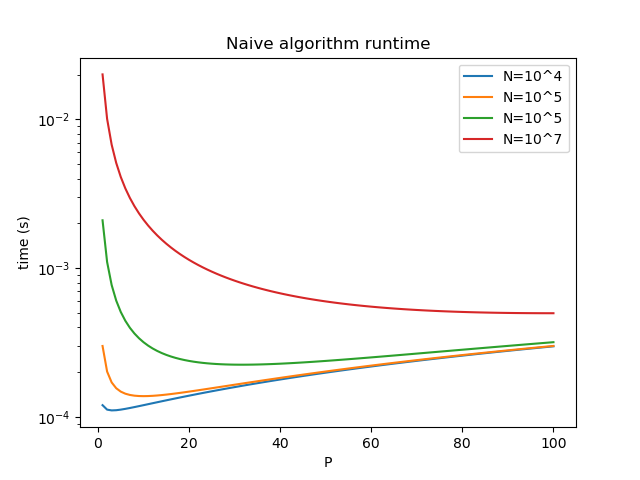
\includegraphics[width=11cm]{theoretical_naive_time}
    \caption{Time of the naive algorithm}
\end{figure}
\begin{figure}[h]
    \includegraphics[width=11cm]{theoretical_naive_scalability}
    \caption{Scalability of the naive algorithm}
\end{figure}
\FloatBarrier
Scalability is not linear; the algorithm scales only when $P$ is small compared to $N$, then scalability peaks and decreases.\\
Optimal scalability is achieved by $N, P_{opt}$ such that $T_{naive}(N, P_{opt})$ is at its mininum given $N$.\\
Ignoring the ceiling on the block size, taking the derivative with respect to $P$ and finding its root $P_{*}$:
$$\frac{\partial T_{naive}(N, P)}{\partial P} = 2T_{comm} + \left(1-\frac{N}{P^{2}}\right)T_{comp}$$
$$2T_{comm} + \left(1-\frac{N}{P_{*}^{2}}\right)T_{comp} = 0$$
$$P_{*} = \sqrt{N\frac{T_{comp}}{2T_{comm} + T_{comp}}}$$
The second derivative is strictly strictly positive, so $P_{*}$ determines a minimum for $T_{naive}$ and a maximum for $S_{naive}$.
$$\frac{\partial^{2} T_{naive}(N, P)}{\partial P^{2}} = \frac{N2T_{comp}}{P^{3}} > 0$$
Recalling $P \geq 1, P \in \mathbb{N}$
$$P_{opt}(N) = \argmin_{P \in \{ \floor{P_{*}}, \ceil{P_{*}} \}, P \geq 1 }{T_{naive}(N, P)} $$\\
The derivative with respect to $N$ is $T_{comp}/P > 0$, there is no stationary point.\\
A different algorithm can be defined, that exploits the system's parallelism by distributing the burden of communications so that they can be performed in parallel, rather than serially by the master.\\
Let the master process have rank $0$ and the slaves have ranks $1$ through $P-1$.\\
Rank $0$ sends to rank $\ceil*{P/2}$, $\floor*{P/2}$ blocks. The problem then reduces to two instances of size $P_{0}=\ceil*{P/2}$ and $P_{1}=\floor*{P/2}$, of which rank $0$ and rank $\ceil*{P/2}$ are the respective masters.\\
The two instances can proceed in parallel until every process either has received a single block, or has sent all but one, at which point computation of the block's sum can be performed.\\
The number of steps required is $\ceil*{\log_{2}(P)}$ and completes in $\ceil*{\log_{2}(P)}T_{comm}$ seconds.\\
Communication of the result will use the opposite of the previous schema, but the message will contain the partial result and the reveicer will sum it with its own; it will complete in $\ceil*{\log_{2}(P)}(T_{comm} + T_{comp})$ seconds.\\
As data are read like in the naive algorithm and each process computes the sum for a block of the same size, the algorithm completes in
$$T_{enh}(N, P) = T_{read} + \ceil*{\log_{2}(P)} (2T_{comm} + T_{comp}) + \left(\frac{N}{P}-1\right)T_{comp}$$
\begin{figure}[h]
    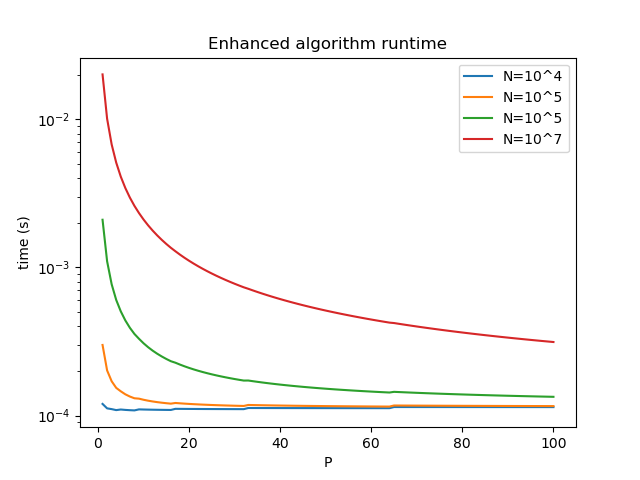
\includegraphics[width=12cm]{theoretical_enhanced_time}
    \caption{Time of the enhanced algorithm}
\end{figure}
\begin{figure}[h]
    \includegraphics[width=12cm]{theoretical_enhanced_scalability}
    \caption{Scalability of the enhanced algorithm}
\end{figure}
\FloatBarrier
The graphs show the effect of the ceiling function, with a sharp increase in time when $P$ passes from a power of 2 to the next integer.\\
Having reduced the communication time to an asymptotically sub-linear function of $P$ greatly benefits the scalability, for which the $P_{opt}(N)$ is linear in $N$.\\
Indeed, relaxing the ceiling function:
$$\frac{\partial T_{enh}(N, P)}{\partial P} = \frac{2T_{comm} + T_{comp}}{\ln(2)P} -\frac{N}{P^{2}} T_{comp}$$
$$\frac{2T_{comm} + T_{comp}}{\ln(2)P_{*}} - \frac{N}{P_{*}^{2}} T_{comp} = 0$$
$$P_{*} = N\ln(2)\frac{T_{comp}}{2T_{comm} + T_{comp}}$$
To reconstruct the condition from the first observation:
$$P_{opt}(N) = \argmin_{P \in \{ 2^{\floor{\log_2(P_{*})}}, 2^{\ceil{\log_2(P_{*})}} \}, P \geq 1}{T_{enh}(N, P)} $$\\
Peak scalability is reached for much greater values of $P$ than with the naive algorithm.\\
\section{MPI program}
Two programs for the estimation of $\pi$ using a Monte-Carlo method have been provided, \texttt{pi.c} and \texttt{mpi\_pi.c}; the first being a serial implementation, the second using MPI.\\
Both programs take as input $N$, the number of iterations.\\
The serial program uses \texttt{clock()} from \texttt{time.h} to measure the processor time elapsed from initialization of the random generator to output of the estimate.\\
The MPI program adopts a master-slave approach where each process computes $\floor{N/P}$ iterations, then each slave sends its result to the master and exits; the master finally computes the estimate. Communications between processes are blocking and the master receives partial sums in sequential order of slaves' ranks.\\
The MPI program uses \texttt{MPI\_Wtime} to measure the elapsed wall time. The master counts from initialization of the random generator to output of the final estimate, thus including the (blocking) receival of each slave's partial sum.\\
Slaves count from initialization of the random generator to the conclusion of the communication to the master.\\
The MPI program is executed through \texttt{mpirun} and it is not possible to make assumptions on the actual starting order of the processes. The extremes of the measured intervals can be interleaved in any possible combination.
\subsection{Strong scalability}

\subsection{Parallel overhead model}

\subsection{Weak scalability}
\end{document}